% GNUPLOT: LaTeX picture with Postscript
\begingroup
  \makeatletter
  \providecommand\color[2][]{%
    \GenericError{(gnuplot) \space\space\space\@spaces}{%
      Package color not loaded in conjunction with
      terminal option `colourtext'%
    }{See the gnuplot documentation for explanation.%
    }{Either use 'blacktext' in gnuplot or load the package
      color.sty in LaTeX.}%
    \renewcommand\color[2][]{}%
  }%
  \providecommand\includegraphics[2][]{%
    \GenericError{(gnuplot) \space\space\space\@spaces}{%
      Package graphicx or graphics not loaded%
    }{See the gnuplot documentation for explanation.%
    }{The gnuplot epslatex terminal needs graphicx.sty or graphics.sty.}%
    \renewcommand\includegraphics[2][]{}%
  }%
  \providecommand\rotatebox[2]{#2}%
  \@ifundefined{ifGPcolor}{%
    \newif\ifGPcolor
    \GPcolorfalse
  }{}%
  \@ifundefined{ifGPblacktext}{%
    \newif\ifGPblacktext
    \GPblacktexttrue
  }{}%
  % define a \g@addto@macro without @ in the name:
  \let\gplgaddtomacro\g@addto@macro
  % define empty templates for all commands taking text:
  \gdef\gplbacktext{}%
  \gdef\gplfronttext{}%
  \makeatother
  \ifGPblacktext
    % no textcolor at all
    \def\colorrgb#1{}%
    \def\colorgray#1{}%
  \else
    % gray or color?
    \ifGPcolor
      \def\colorrgb#1{\color[rgb]{#1}}%
      \def\colorgray#1{\color[gray]{#1}}%
      \expandafter\def\csname LTw\endcsname{\color{white}}%
      \expandafter\def\csname LTb\endcsname{\color{black}}%
      \expandafter\def\csname LTa\endcsname{\color{black}}%
      \expandafter\def\csname LT0\endcsname{\color[rgb]{1,0,0}}%
      \expandafter\def\csname LT1\endcsname{\color[rgb]{0,1,0}}%
      \expandafter\def\csname LT2\endcsname{\color[rgb]{0,0,1}}%
      \expandafter\def\csname LT3\endcsname{\color[rgb]{1,0,1}}%
      \expandafter\def\csname LT4\endcsname{\color[rgb]{0,1,1}}%
      \expandafter\def\csname LT5\endcsname{\color[rgb]{1,1,0}}%
      \expandafter\def\csname LT6\endcsname{\color[rgb]{0,0,0}}%
      \expandafter\def\csname LT7\endcsname{\color[rgb]{1,0.3,0}}%
      \expandafter\def\csname LT8\endcsname{\color[rgb]{0.5,0.5,0.5}}%
    \else
      % gray
      \def\colorrgb#1{\color{black}}%
      \def\colorgray#1{\color[gray]{#1}}%
      \expandafter\def\csname LTw\endcsname{\color{white}}%
      \expandafter\def\csname LTb\endcsname{\color{black}}%
      \expandafter\def\csname LTa\endcsname{\color{black}}%
      \expandafter\def\csname LT0\endcsname{\color{black}}%
      \expandafter\def\csname LT1\endcsname{\color{black}}%
      \expandafter\def\csname LT2\endcsname{\color{black}}%
      \expandafter\def\csname LT3\endcsname{\color{black}}%
      \expandafter\def\csname LT4\endcsname{\color{black}}%
      \expandafter\def\csname LT5\endcsname{\color{black}}%
      \expandafter\def\csname LT6\endcsname{\color{black}}%
      \expandafter\def\csname LT7\endcsname{\color{black}}%
      \expandafter\def\csname LT8\endcsname{\color{black}}%
    \fi
  \fi
  \setlength{\unitlength}{0.0500bp}%
  \begin{picture}(8502.00,6802.00)%
      \csname LTb\endcsname%
      \put(4251,6582){\makebox(0,0){\strut{}Rechteckspannung mit $f=100Hz$}}%
    \gplgaddtomacro\gplbacktext{%
      \csname LTb\endcsname%
      \put(946,3995){\makebox(0,0)[r]{\strut{}-0.6}}%
      \put(946,4316){\makebox(0,0)[r]{\strut{}-0.4}}%
      \put(946,4637){\makebox(0,0)[r]{\strut{}-0.2}}%
      \put(946,4958){\makebox(0,0)[r]{\strut{} 0}}%
      \put(946,5279){\makebox(0,0)[r]{\strut{} 0.2}}%
      \put(946,5600){\makebox(0,0)[r]{\strut{} 0.4}}%
      \put(946,5921){\makebox(0,0)[r]{\strut{} 0.6}}%
      \put(1078,3775){\makebox(0,0){\strut{} 0}}%
      \put(2483,3775){\makebox(0,0){\strut{} 0.05}}%
      \put(3889,3775){\makebox(0,0){\strut{} 0.1}}%
      \put(5294,3775){\makebox(0,0){\strut{} 0.15}}%
      \put(6700,3775){\makebox(0,0){\strut{} 0.2}}%
      \put(8105,3775){\makebox(0,0){\strut{} 0.25}}%
      \put(176,4958){\rotatebox{-270}{\makebox(0,0){\strut{}$U \ [V]$}}}%
      \put(4591,3445){\makebox(0,0){\strut{}$t \ [s]$}}%
      \put(4591,6251){\makebox(0,0){\strut{}Zeitverlauf}}%
    }%
    \gplgaddtomacro\gplfronttext{%
    }%
    \gplgaddtomacro\gplbacktext{%
      \csname LTb\endcsname%
      \put(1078,704){\makebox(0,0)[r]{\strut{} 0}}%
      \put(1078,897){\makebox(0,0)[r]{\strut{} 0.05}}%
      \put(1078,1089){\makebox(0,0)[r]{\strut{} 0.1}}%
      \put(1078,1282){\makebox(0,0)[r]{\strut{} 0.15}}%
      \put(1078,1475){\makebox(0,0)[r]{\strut{} 0.2}}%
      \put(1078,1668){\makebox(0,0)[r]{\strut{} 0.25}}%
      \put(1078,1860){\makebox(0,0)[r]{\strut{} 0.3}}%
      \put(1078,2053){\makebox(0,0)[r]{\strut{} 0.35}}%
      \put(1078,2246){\makebox(0,0)[r]{\strut{} 0.4}}%
      \put(1078,2438){\makebox(0,0)[r]{\strut{} 0.45}}%
      \put(1078,2631){\makebox(0,0)[r]{\strut{} 0.5}}%
      \put(1210,484){\makebox(0,0){\strut{} 0}}%
      \put(1900,484){\makebox(0,0){\strut{} 500}}%
      \put(2589,484){\makebox(0,0){\strut{} 1000}}%
      \put(3279,484){\makebox(0,0){\strut{} 1500}}%
      \put(3968,484){\makebox(0,0){\strut{} 2000}}%
      \put(4658,484){\makebox(0,0){\strut{} 2500}}%
      \put(5347,484){\makebox(0,0){\strut{} 3000}}%
      \put(6037,484){\makebox(0,0){\strut{} 3500}}%
      \put(6726,484){\makebox(0,0){\strut{} 4000}}%
      \put(7416,484){\makebox(0,0){\strut{} 4500}}%
      \put(8105,484){\makebox(0,0){\strut{} 5000}}%
      \put(176,1667){\rotatebox{-270}{\makebox(0,0){\strut{}$F$}}}%
      \put(4657,154){\makebox(0,0){\strut{}$f \ [Hz]$}}%
      \put(4657,2961){\makebox(0,0){\strut{}Frequenzspektrum}}%
    }%
    \gplgaddtomacro\gplfronttext{%
    }%
    \gplbacktext
    \put(0,0){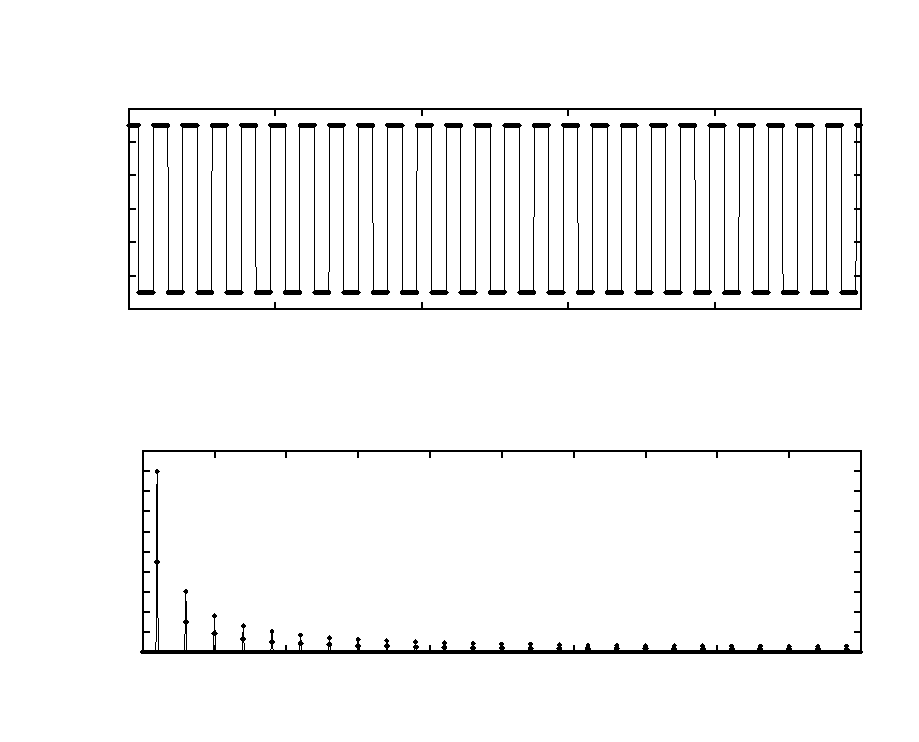
\includegraphics{1-rechteck}}%
    \gplfronttext
  \end{picture}%
\endgroup
